% Options for packages loaded elsewhere
\PassOptionsToPackage{unicode}{hyperref}
\PassOptionsToPackage{hyphens}{url}
%
\documentclass[
]{article}
\usepackage{lmodern}
\usepackage{amsmath}
\usepackage{ifxetex,ifluatex}
\ifnum 0\ifxetex 1\fi\ifluatex 1\fi=0 % if pdftex
  \usepackage[T1]{fontenc}
  \usepackage[utf8]{inputenc}
  \usepackage{textcomp} % provide euro and other symbols
  \usepackage{amssymb}
\else % if luatex or xetex
  \usepackage{unicode-math}
  \defaultfontfeatures{Scale=MatchLowercase}
  \defaultfontfeatures[\rmfamily]{Ligatures=TeX,Scale=1}
\fi
% Use upquote if available, for straight quotes in verbatim environments
\IfFileExists{upquote.sty}{\usepackage{upquote}}{}
\IfFileExists{microtype.sty}{% use microtype if available
  \usepackage[]{microtype}
  \UseMicrotypeSet[protrusion]{basicmath} % disable protrusion for tt fonts
}{}
\makeatletter
\@ifundefined{KOMAClassName}{% if non-KOMA class
  \IfFileExists{parskip.sty}{%
    \usepackage{parskip}
  }{% else
    \setlength{\parindent}{0pt}
    \setlength{\parskip}{6pt plus 2pt minus 1pt}}
}{% if KOMA class
  \KOMAoptions{parskip=half}}
\makeatother
\usepackage{xcolor}
\IfFileExists{xurl.sty}{\usepackage{xurl}}{} % add URL line breaks if available
\IfFileExists{bookmark.sty}{\usepackage{bookmark}}{\usepackage{hyperref}}
\hypersetup{
  pdftitle={hw3},
  pdfauthor={Enbo Tian},
  hidelinks,
  pdfcreator={LaTeX via pandoc}}
\urlstyle{same} % disable monospaced font for URLs
\usepackage[margin=1in]{geometry}
\usepackage{color}
\usepackage{fancyvrb}
\newcommand{\VerbBar}{|}
\newcommand{\VERB}{\Verb[commandchars=\\\{\}]}
\DefineVerbatimEnvironment{Highlighting}{Verbatim}{commandchars=\\\{\}}
% Add ',fontsize=\small' for more characters per line
\usepackage{framed}
\definecolor{shadecolor}{RGB}{248,248,248}
\newenvironment{Shaded}{\begin{snugshade}}{\end{snugshade}}
\newcommand{\AlertTok}[1]{\textcolor[rgb]{0.94,0.16,0.16}{#1}}
\newcommand{\AnnotationTok}[1]{\textcolor[rgb]{0.56,0.35,0.01}{\textbf{\textit{#1}}}}
\newcommand{\AttributeTok}[1]{\textcolor[rgb]{0.77,0.63,0.00}{#1}}
\newcommand{\BaseNTok}[1]{\textcolor[rgb]{0.00,0.00,0.81}{#1}}
\newcommand{\BuiltInTok}[1]{#1}
\newcommand{\CharTok}[1]{\textcolor[rgb]{0.31,0.60,0.02}{#1}}
\newcommand{\CommentTok}[1]{\textcolor[rgb]{0.56,0.35,0.01}{\textit{#1}}}
\newcommand{\CommentVarTok}[1]{\textcolor[rgb]{0.56,0.35,0.01}{\textbf{\textit{#1}}}}
\newcommand{\ConstantTok}[1]{\textcolor[rgb]{0.00,0.00,0.00}{#1}}
\newcommand{\ControlFlowTok}[1]{\textcolor[rgb]{0.13,0.29,0.53}{\textbf{#1}}}
\newcommand{\DataTypeTok}[1]{\textcolor[rgb]{0.13,0.29,0.53}{#1}}
\newcommand{\DecValTok}[1]{\textcolor[rgb]{0.00,0.00,0.81}{#1}}
\newcommand{\DocumentationTok}[1]{\textcolor[rgb]{0.56,0.35,0.01}{\textbf{\textit{#1}}}}
\newcommand{\ErrorTok}[1]{\textcolor[rgb]{0.64,0.00,0.00}{\textbf{#1}}}
\newcommand{\ExtensionTok}[1]{#1}
\newcommand{\FloatTok}[1]{\textcolor[rgb]{0.00,0.00,0.81}{#1}}
\newcommand{\FunctionTok}[1]{\textcolor[rgb]{0.00,0.00,0.00}{#1}}
\newcommand{\ImportTok}[1]{#1}
\newcommand{\InformationTok}[1]{\textcolor[rgb]{0.56,0.35,0.01}{\textbf{\textit{#1}}}}
\newcommand{\KeywordTok}[1]{\textcolor[rgb]{0.13,0.29,0.53}{\textbf{#1}}}
\newcommand{\NormalTok}[1]{#1}
\newcommand{\OperatorTok}[1]{\textcolor[rgb]{0.81,0.36,0.00}{\textbf{#1}}}
\newcommand{\OtherTok}[1]{\textcolor[rgb]{0.56,0.35,0.01}{#1}}
\newcommand{\PreprocessorTok}[1]{\textcolor[rgb]{0.56,0.35,0.01}{\textit{#1}}}
\newcommand{\RegionMarkerTok}[1]{#1}
\newcommand{\SpecialCharTok}[1]{\textcolor[rgb]{0.00,0.00,0.00}{#1}}
\newcommand{\SpecialStringTok}[1]{\textcolor[rgb]{0.31,0.60,0.02}{#1}}
\newcommand{\StringTok}[1]{\textcolor[rgb]{0.31,0.60,0.02}{#1}}
\newcommand{\VariableTok}[1]{\textcolor[rgb]{0.00,0.00,0.00}{#1}}
\newcommand{\VerbatimStringTok}[1]{\textcolor[rgb]{0.31,0.60,0.02}{#1}}
\newcommand{\WarningTok}[1]{\textcolor[rgb]{0.56,0.35,0.01}{\textbf{\textit{#1}}}}
\usepackage{graphicx}
\makeatletter
\def\maxwidth{\ifdim\Gin@nat@width>\linewidth\linewidth\else\Gin@nat@width\fi}
\def\maxheight{\ifdim\Gin@nat@height>\textheight\textheight\else\Gin@nat@height\fi}
\makeatother
% Scale images if necessary, so that they will not overflow the page
% margins by default, and it is still possible to overwrite the defaults
% using explicit options in \includegraphics[width, height, ...]{}
\setkeys{Gin}{width=\maxwidth,height=\maxheight,keepaspectratio}
% Set default figure placement to htbp
\makeatletter
\def\fps@figure{htbp}
\makeatother
\setlength{\emergencystretch}{3em} % prevent overfull lines
\providecommand{\tightlist}{%
  \setlength{\itemsep}{0pt}\setlength{\parskip}{0pt}}
\setcounter{secnumdepth}{-\maxdimen} % remove section numbering
\ifluatex
  \usepackage{selnolig}  % disable illegal ligatures
\fi

\title{hw3}
\author{Enbo Tian}
\date{2022/2/28}

\begin{document}
\maketitle

\hypertarget{graphical-model-1}{%
\section{Graphical Model 1}\label{graphical-model-1}}

\hypertarget{a}{%
\subsection{a)}\label{a}}

\begin{Shaded}
\begin{Highlighting}[]
\FunctionTok{rm}\NormalTok{(}\AttributeTok{list =} \FunctionTok{ls}\NormalTok{())}
\NormalTok{X }\OtherTok{\textless{}{-}} \FunctionTok{c}\NormalTok{(}\StringTok{"cold"}\NormalTok{, }\StringTok{"hot"}\NormalTok{, }\StringTok{"mild"}\NormalTok{)}
\CommentTok{\# day 0}
\NormalTok{day0 }\OtherTok{=} \FunctionTok{replicate}\NormalTok{(}\DecValTok{5}\NormalTok{,}\FunctionTok{sample}\NormalTok{(X,}\AttributeTok{size =} \DecValTok{1}\NormalTok{,}\AttributeTok{prob=}\FunctionTok{c}\NormalTok{(}\DecValTok{1}\SpecialCharTok{/}\DecValTok{3}\NormalTok{,}\DecValTok{1}\SpecialCharTok{/}\DecValTok{3}\NormalTok{,}\DecValTok{1}\SpecialCharTok{/}\DecValTok{3}\NormalTok{)))}
\CommentTok{\# function of day}
\NormalTok{dayk }\OtherTok{\textless{}{-}} \ControlFlowTok{function}\NormalTok{(day)\{}
\NormalTok{  dayk }\OtherTok{\textless{}{-}} \FunctionTok{rep}\NormalTok{(}\DecValTok{0}\NormalTok{,}\DecValTok{5}\NormalTok{)}
  \ControlFlowTok{for}\NormalTok{ (i }\ControlFlowTok{in} \DecValTok{1}\SpecialCharTok{:}\DecValTok{5}\NormalTok{)\{}
    \ControlFlowTok{if}\NormalTok{ (day[i] }\SpecialCharTok{==} \StringTok{"cold"}\NormalTok{)\{}
\NormalTok{    dayk[i] }\OtherTok{=} \FunctionTok{sample}\NormalTok{(}\FunctionTok{c}\NormalTok{(}\StringTok{"cold"}\NormalTok{, }\StringTok{"hot"}\NormalTok{, }\StringTok{"mild"}\NormalTok{),}\AttributeTok{size =}\DecValTok{1}\NormalTok{,}\AttributeTok{prob =} \FunctionTok{c}\NormalTok{(}\DecValTok{1}\SpecialCharTok{/}\DecValTok{2}\NormalTok{,}\DecValTok{1}\SpecialCharTok{/}\DecValTok{4}\NormalTok{,}\DecValTok{1}\SpecialCharTok{/}\DecValTok{4}\NormalTok{))}
\NormalTok{    \}}
    \ControlFlowTok{else} \ControlFlowTok{if}\NormalTok{ (day[i] }\SpecialCharTok{==} \StringTok{"hot"}\NormalTok{)\{}
\NormalTok{    dayk[i] }\OtherTok{=} \FunctionTok{sample}\NormalTok{(}\FunctionTok{c}\NormalTok{(}\StringTok{"cold"}\NormalTok{, }\StringTok{"hot"}\NormalTok{, }\StringTok{"mild"}\NormalTok{),}\AttributeTok{size =}\DecValTok{1}\NormalTok{,}\AttributeTok{prob =} \FunctionTok{c}\NormalTok{(}\DecValTok{1}\SpecialCharTok{/}\DecValTok{3}\NormalTok{,}\DecValTok{1}\SpecialCharTok{/}\DecValTok{3}\NormalTok{,}\DecValTok{1}\SpecialCharTok{/}\DecValTok{3}\NormalTok{))}
\NormalTok{    \}}
    \ControlFlowTok{else} \ControlFlowTok{if}\NormalTok{(day[i] }\SpecialCharTok{==} \StringTok{"mild"}\NormalTok{)\{}
\NormalTok{      dayk[i]}\OtherTok{=} \FunctionTok{sample}\NormalTok{(}\FunctionTok{c}\NormalTok{(}\StringTok{"cold"}\NormalTok{, }\StringTok{"hot"}\NormalTok{, }\StringTok{"mild"}\NormalTok{),}\AttributeTok{size =}\DecValTok{1}\NormalTok{,}\AttributeTok{prob =} \FunctionTok{c}\NormalTok{(}\DecValTok{1}\SpecialCharTok{/}\DecValTok{4}\NormalTok{,}\DecValTok{1}\SpecialCharTok{/}\DecValTok{4}\NormalTok{,}\DecValTok{1}\SpecialCharTok{/}\DecValTok{2}\NormalTok{))}
\NormalTok{    \}}
\NormalTok{  \}}
\NormalTok{  dayk}
\NormalTok{\}}
\CommentTok{\# day 1:5}
\NormalTok{day1 }\OtherTok{\textless{}{-}} \FunctionTok{dayk}\NormalTok{(day0)}
\NormalTok{day2 }\OtherTok{\textless{}{-}} \FunctionTok{dayk}\NormalTok{(day1)}
\NormalTok{day3 }\OtherTok{\textless{}{-}} \FunctionTok{dayk}\NormalTok{(day2)}
\NormalTok{day4 }\OtherTok{\textless{}{-}} \FunctionTok{dayk}\NormalTok{(day3)}

\NormalTok{day }\OtherTok{\textless{}{-}} \FunctionTok{data.frame}\NormalTok{(day0, day1, day2, day3, day4)}
\NormalTok{day}
\end{Highlighting}
\end{Shaded}

\begin{verbatim}
##   day0 day1 day2 day3 day4
## 1 cold mild  hot mild cold
## 2  hot cold mild mild mild
## 3 mild mild mild mild mild
## 4 mild mild mild mild  hot
## 5  hot mild mild mild  hot
\end{verbatim}

\hypertarget{b}{%
\subsection{b)}\label{b}}

\begin{Shaded}
\begin{Highlighting}[]
\CommentTok{\# P(day0)}
\NormalTok{p0 }\OtherTok{\textless{}{-}} \FunctionTok{c}\NormalTok{(}\DecValTok{1}\SpecialCharTok{/}\DecValTok{3}\NormalTok{,}\DecValTok{1}\SpecialCharTok{/}\DecValTok{3}\NormalTok{,}\DecValTok{1}\SpecialCharTok{/}\DecValTok{3}\NormalTok{)}
\CommentTok{\# p (k given k{-}1)}
\NormalTok{pgiven }\OtherTok{\textless{}{-}} \FunctionTok{matrix}\NormalTok{(}\FunctionTok{c}\NormalTok{(}\DecValTok{1}\SpecialCharTok{/}\DecValTok{2}\NormalTok{,}\DecValTok{1}\SpecialCharTok{/}\DecValTok{4}\NormalTok{,}\DecValTok{1}\SpecialCharTok{/}\DecValTok{4}\NormalTok{,}\DecValTok{1}\SpecialCharTok{/}\DecValTok{3}\NormalTok{,}\DecValTok{1}\SpecialCharTok{/}\DecValTok{3}\NormalTok{,}\DecValTok{1}\SpecialCharTok{/}\DecValTok{3}\NormalTok{,}\DecValTok{1}\SpecialCharTok{/}\DecValTok{4}\NormalTok{,}\DecValTok{1}\SpecialCharTok{/}\DecValTok{4}\NormalTok{,}\DecValTok{1}\SpecialCharTok{/}\DecValTok{2}\NormalTok{),}\AttributeTok{ncol=}\DecValTok{3}\NormalTok{)}
\CommentTok{\# marginal prob}
\NormalTok{p1 }\OtherTok{\textless{}{-}}\NormalTok{ pgiven}\SpecialCharTok{\%*\%}\NormalTok{p0}
\NormalTok{p2 }\OtherTok{\textless{}{-}}\NormalTok{ pgiven}\SpecialCharTok{\%*\%}\NormalTok{p1}
\NormalTok{p3 }\OtherTok{\textless{}{-}}\NormalTok{ pgiven}\SpecialCharTok{\%*\%}\NormalTok{p2}
\NormalTok{margp }\OtherTok{\textless{}{-}} \FunctionTok{data.frame}\NormalTok{(p0,p1,p2,p3)}
\NormalTok{margp}
\end{Highlighting}
\end{Shaded}

\begin{verbatim}
##          p0        p1        p2        p3
## 1 0.3333333 0.3611111 0.3634259 0.3636188
## 2 0.3333333 0.2777778 0.2731481 0.2727623
## 3 0.3333333 0.3611111 0.3634259 0.3636188
\end{verbatim}

\hypertarget{c}{%
\subsection{c)}\label{c}}

\begin{Shaded}
\begin{Highlighting}[]
\CommentTok{\# 3|2hot }
\NormalTok{p3g2 }\OtherTok{\textless{}{-}} \FunctionTok{c}\NormalTok{(}\DecValTok{1}\SpecialCharTok{/}\DecValTok{3}\NormalTok{,}\DecValTok{1}\SpecialCharTok{/}\DecValTok{3}\NormalTok{,}\DecValTok{1}\SpecialCharTok{/}\DecValTok{3}\NormalTok{)}
\NormalTok{p3g2}
\end{Highlighting}
\end{Shaded}

\begin{verbatim}
## [1] 0.3333333 0.3333333 0.3333333
\end{verbatim}

\begin{Shaded}
\begin{Highlighting}[]
\CommentTok{\# p(1|2="hot") = p(2|1)*p(1)/p(2 = "hot")}
\NormalTok{p1 }\OtherTok{\textless{}{-}} \FunctionTok{c}\NormalTok{(p1)}
\NormalTok{p2 }\OtherTok{\textless{}{-}} \FunctionTok{c}\NormalTok{(p2)}
\NormalTok{p3 }\OtherTok{\textless{}{-}} \FunctionTok{c}\NormalTok{(p3)}
\NormalTok{p1g2 }\OtherTok{\textless{}{-}}\NormalTok{ pgiven }\SpecialCharTok{*}\NormalTok{ p1 }\SpecialCharTok{/}\NormalTok{ p2 }
\NormalTok{p1g2 }\OtherTok{\textless{}{-}} \FunctionTok{c}\NormalTok{(p1g2[,}\DecValTok{2}\NormalTok{])}
\NormalTok{p1g2}
\end{Highlighting}
\end{Shaded}

\begin{verbatim}
## [1] 0.3312102 0.3389831 0.3312102
\end{verbatim}

\begin{Shaded}
\begin{Highlighting}[]
\CommentTok{\# p(0|1) = p(1|0)*p(0)/p(1|2="hot")}
\NormalTok{p0g1 }\OtherTok{\textless{}{-}}\NormalTok{ pgiven }\SpecialCharTok{*}\NormalTok{ p0 }\SpecialCharTok{/}\NormalTok{p1g2}
\NormalTok{p0g1}
\end{Highlighting}
\end{Shaded}

\begin{verbatim}
##           [,1]      [,2]      [,3]
## [1,] 0.5032051 0.3354701 0.2516026
## [2,] 0.2458333 0.3277778 0.2458333
## [3,] 0.2516026 0.3354701 0.5032051
\end{verbatim}

\hypertarget{d}{%
\subsection{d)}\label{d}}

\begin{Shaded}
\begin{Highlighting}[]
\CommentTok{\# give day2 is hot}
\NormalTok{day2 }\OtherTok{=} \StringTok{"hot"}
\CommentTok{\# get most probable day1}
\ControlFlowTok{if}\NormalTok{ (}\FunctionTok{max}\NormalTok{(p1g2) }\SpecialCharTok{==}\NormalTok{ p1g2[}\DecValTok{1}\NormalTok{])\{}
\NormalTok{  day1 }\OtherTok{=} \StringTok{"cold"}
\NormalTok{  i }\OtherTok{=} \DecValTok{1}
\NormalTok{\}}\ControlFlowTok{else} \ControlFlowTok{if}\NormalTok{(}\FunctionTok{max}\NormalTok{(p1g2) }\SpecialCharTok{==}\NormalTok{ p1g2[}\DecValTok{2}\NormalTok{])\{}
\NormalTok{  day1 }\OtherTok{=} \StringTok{"hot"}
\NormalTok{  i }\OtherTok{=} \DecValTok{2}
\NormalTok{\}}\ControlFlowTok{else} \ControlFlowTok{if}\NormalTok{(}\FunctionTok{max}\NormalTok{(p1g2) }\SpecialCharTok{==}\NormalTok{ p1g2[}\DecValTok{3}\NormalTok{])\{}
\NormalTok{  day1 }\OtherTok{=} \StringTok{"mild"}
\NormalTok{  i }\OtherTok{=}\DecValTok{3}
\NormalTok{\}}
\CommentTok{\# get most probable day0}
\NormalTok{new\_p0g1 }\OtherTok{\textless{}{-}}\NormalTok{ p0g1[,i]}
\ControlFlowTok{if}\NormalTok{ (}\FunctionTok{max}\NormalTok{(new\_p0g1) }\SpecialCharTok{==}\NormalTok{ new\_p0g1[}\DecValTok{1}\NormalTok{])\{}
\NormalTok{  day0 }\OtherTok{=} \StringTok{"cold"}
\NormalTok{\}}\ControlFlowTok{else} \ControlFlowTok{if}\NormalTok{(}\FunctionTok{max}\NormalTok{(new\_p0g1) }\SpecialCharTok{==}\NormalTok{ new\_p0g1[}\DecValTok{2}\NormalTok{])\{}
\NormalTok{  day0 }\OtherTok{=} \StringTok{"hot"}
\NormalTok{\}}\ControlFlowTok{else} \ControlFlowTok{if}\NormalTok{(}\FunctionTok{max}\NormalTok{(new\_p0g1) }\SpecialCharTok{==}\NormalTok{ new\_p0g1[}\DecValTok{3}\NormalTok{])\{}
\NormalTok{  day0 }\OtherTok{=} \StringTok{"mild"}
\NormalTok{\}}
\CommentTok{\# Same prob for day3 given hot of day2}
\FunctionTok{c}\NormalTok{(day0,day1,day2)}
\end{Highlighting}
\end{Shaded}

\begin{verbatim}
## [1] "cold" "hot"  "hot"
\end{verbatim}

the most probable report for day 0 to 2 are ``cold'' ``hot'' ``hot'',
and

we have the same probability for day3.

\hypertarget{graphical-model-2}{%
\section{Graphical Model 2}\label{graphical-model-2}}

\hypertarget{a-1}{%
\subsection{a)}\label{a-1}}

\begin{Shaded}
\begin{Highlighting}[]
\NormalTok{mi }\OtherTok{\textless{}{-}} \FunctionTok{c}\NormalTok{(}\SpecialCharTok{{-}}\DecValTok{2}\NormalTok{, }\DecValTok{2}\NormalTok{ ,}\DecValTok{0}\NormalTok{)}
\CommentTok{\# height function}
\NormalTok{height }\OtherTok{\textless{}{-}} \ControlFlowTok{function}\NormalTok{(statep)\{}
\NormalTok{  m }\OtherTok{\textless{}{-}} \FunctionTok{replicate}\NormalTok{(}\DecValTok{5}\NormalTok{,}\FunctionTok{sample}\NormalTok{(mi,}\AttributeTok{size =} \DecValTok{1}\NormalTok{,}\AttributeTok{prob =}\NormalTok{ statep))}
\NormalTok{  y }\OtherTok{\textless{}{-}} \FunctionTok{rep}\NormalTok{(}\DecValTok{0}\NormalTok{,}\DecValTok{5}\NormalTok{)}
  \ControlFlowTok{for}\NormalTok{ (i }\ControlFlowTok{in} \DecValTok{1}\SpecialCharTok{:}\DecValTok{5}\NormalTok{)\{}
\NormalTok{    y[i] }\OtherTok{\textless{}{-}} \FunctionTok{rnorm}\NormalTok{(}\DecValTok{1}\NormalTok{,m,}\DecValTok{1}\NormalTok{)}
\NormalTok{  \}}
\NormalTok{  y}
\NormalTok{\}}
\CommentTok{\# get height}
\NormalTok{y0 }\OtherTok{\textless{}{-}} \FunctionTok{height}\NormalTok{(p0)}
\NormalTok{y1 }\OtherTok{\textless{}{-}} \FunctionTok{height}\NormalTok{(p1)}
\NormalTok{y2 }\OtherTok{\textless{}{-}} \FunctionTok{height}\NormalTok{(p2)}
\NormalTok{y3 }\OtherTok{\textless{}{-}} \FunctionTok{height}\NormalTok{(p3)}
\NormalTok{datay }\OtherTok{\textless{}{-}} \FunctionTok{data.frame}\NormalTok{(y0,y1,y2,y3)}
\NormalTok{datay}
\end{Highlighting}
\end{Shaded}

\begin{verbatim}
##          y0         y1         y2          y3
## 1 1.1846050 -2.6583488 -1.2333962 -0.48188241
## 2 2.6422173  1.5165965  0.8667888 -1.15463369
## 3 0.7535893  1.4933726  0.3648090 -0.75774038
## 4 2.6192513 -1.4818251 -0.6577560  0.45392296
## 5 1.1178091 -0.4164611  0.8649524  0.06917906
\end{verbatim}

\hypertarget{b-1}{%
\subsection{b)}\label{b-1}}

\begin{Shaded}
\begin{Highlighting}[]
\NormalTok{m }\OtherTok{\textless{}{-}} \FunctionTok{c}\NormalTok{(}\DecValTok{2}\NormalTok{,}\DecValTok{0}\NormalTok{,}\SpecialCharTok{{-}}\DecValTok{2}\NormalTok{,}\SpecialCharTok{{-}}\DecValTok{2}\NormalTok{)}
\NormalTok{y0 }\OtherTok{\textless{}{-}}\FunctionTok{replicate}\NormalTok{(}\DecValTok{5}\NormalTok{,}\FunctionTok{rnorm}\NormalTok{(}\DecValTok{1}\NormalTok{,m[}\DecValTok{1}\NormalTok{],}\DecValTok{1}\NormalTok{)) }
\NormalTok{y1 }\OtherTok{\textless{}{-}}\FunctionTok{replicate}\NormalTok{(}\DecValTok{5}\NormalTok{,}\FunctionTok{rnorm}\NormalTok{(}\DecValTok{1}\NormalTok{,m[}\DecValTok{2}\NormalTok{],}\DecValTok{1}\NormalTok{))}
\NormalTok{y2 }\OtherTok{\textless{}{-}}\FunctionTok{replicate}\NormalTok{(}\DecValTok{5}\NormalTok{,}\FunctionTok{rnorm}\NormalTok{(}\DecValTok{1}\NormalTok{,m[}\DecValTok{3}\NormalTok{],}\DecValTok{1}\NormalTok{))}
\NormalTok{y3 }\OtherTok{\textless{}{-}}\FunctionTok{replicate}\NormalTok{(}\DecValTok{5}\NormalTok{,}\FunctionTok{rnorm}\NormalTok{(}\DecValTok{1}\NormalTok{,m[}\DecValTok{4}\NormalTok{],}\DecValTok{1}\NormalTok{))}
\NormalTok{data2y}\OtherTok{\textless{}{-}} \FunctionTok{data.frame}\NormalTok{(y0,y1,y2,y3)}
\NormalTok{data2y}
\end{Highlighting}
\end{Shaded}

\begin{verbatim}
##          y0         y1         y2         y3
## 1 1.7206229 -2.3802289 -2.8862296 -0.5808817
## 2 3.3414048  0.2461311 -2.0892577 -2.4564032
## 3 3.3789101 -0.3644545 -0.6326099 -0.8114039
## 4 0.5745347 -0.5117749 -1.8682332 -1.9761502
## 5 2.9935593 -0.6412759 -2.1486982 -1.2411396
\end{verbatim}

\hypertarget{c-1}{%
\subsection{c)}\label{c-1}}

\begin{Shaded}
\begin{Highlighting}[]
\NormalTok{Y0 }\OtherTok{=}\FloatTok{0.7}
\NormalTok{Y1 }\OtherTok{=}\FloatTok{1.5}
\NormalTok{Y2 }\OtherTok{=}\SpecialCharTok{{-}}\FloatTok{1.8}
\NormalTok{Y3 }\OtherTok{=}\SpecialCharTok{{-}}\DecValTok{1}

\CommentTok{\#p(y0|x0)}
\NormalTok{d0 }\OtherTok{\textless{}{-}} \FunctionTok{rep}\NormalTok{(}\DecValTok{0}\NormalTok{,}\DecValTok{3}\NormalTok{)}
\NormalTok{d0[}\DecValTok{1}\NormalTok{] }\OtherTok{\textless{}{-}} \FunctionTok{dnorm}\NormalTok{(Y0,}\SpecialCharTok{{-}}\DecValTok{2}\NormalTok{,}\DecValTok{1}\NormalTok{)}
\NormalTok{d0[}\DecValTok{2}\NormalTok{] }\OtherTok{\textless{}{-}} \FunctionTok{dnorm}\NormalTok{(Y0,}\DecValTok{0}\NormalTok{,}\DecValTok{1}\NormalTok{)}
\NormalTok{d0[}\DecValTok{3}\NormalTok{] }\OtherTok{\textless{}{-}} \FunctionTok{dnorm}\NormalTok{(Y0,}\DecValTok{2}\NormalTok{,}\DecValTok{1}\NormalTok{)}
\CommentTok{\#p(y1|x1)}
\NormalTok{d1 }\OtherTok{\textless{}{-}} \FunctionTok{rep}\NormalTok{(}\DecValTok{0}\NormalTok{,}\DecValTok{3}\NormalTok{)}
\NormalTok{d1[}\DecValTok{1}\NormalTok{] }\OtherTok{\textless{}{-}} \FunctionTok{dnorm}\NormalTok{(Y1,}\SpecialCharTok{{-}}\DecValTok{2}\NormalTok{,}\DecValTok{1}\NormalTok{)}
\NormalTok{d1[}\DecValTok{2}\NormalTok{] }\OtherTok{\textless{}{-}} \FunctionTok{dnorm}\NormalTok{(Y1,}\DecValTok{0}\NormalTok{,}\DecValTok{1}\NormalTok{)}
\NormalTok{d1[}\DecValTok{3}\NormalTok{] }\OtherTok{\textless{}{-}} \FunctionTok{dnorm}\NormalTok{(Y1,}\DecValTok{2}\NormalTok{,}\DecValTok{1}\NormalTok{)}
\CommentTok{\#p(y2|x2)}
\NormalTok{d2 }\OtherTok{\textless{}{-}} \FunctionTok{rep}\NormalTok{(}\DecValTok{0}\NormalTok{,}\DecValTok{3}\NormalTok{)}
\NormalTok{d2[}\DecValTok{1}\NormalTok{] }\OtherTok{\textless{}{-}} \FunctionTok{dnorm}\NormalTok{(Y2,}\SpecialCharTok{{-}}\DecValTok{2}\NormalTok{,}\DecValTok{1}\NormalTok{)}
\NormalTok{d2[}\DecValTok{2}\NormalTok{] }\OtherTok{\textless{}{-}} \FunctionTok{dnorm}\NormalTok{(Y2,}\DecValTok{0}\NormalTok{,}\DecValTok{1}\NormalTok{)}
\NormalTok{d2[}\DecValTok{3}\NormalTok{] }\OtherTok{\textless{}{-}} \FunctionTok{dnorm}\NormalTok{(Y2,}\DecValTok{2}\NormalTok{,}\DecValTok{1}\NormalTok{)}
\CommentTok{\#p(y1|x1)}
\NormalTok{d3 }\OtherTok{\textless{}{-}} \FunctionTok{rep}\NormalTok{(}\DecValTok{0}\NormalTok{,}\DecValTok{3}\NormalTok{)}
\NormalTok{d3[}\DecValTok{1}\NormalTok{] }\OtherTok{\textless{}{-}} \FunctionTok{dnorm}\NormalTok{(Y3,}\SpecialCharTok{{-}}\DecValTok{2}\NormalTok{,}\DecValTok{1}\NormalTok{)}
\NormalTok{d3[}\DecValTok{2}\NormalTok{] }\OtherTok{\textless{}{-}} \FunctionTok{dnorm}\NormalTok{(Y3,}\DecValTok{0}\NormalTok{,}\DecValTok{1}\NormalTok{)}
\NormalTok{d3[}\DecValTok{3}\NormalTok{] }\OtherTok{\textless{}{-}} \FunctionTok{dnorm}\NormalTok{(Y3,}\DecValTok{2}\NormalTok{,}\DecValTok{1}\NormalTok{)}
\CommentTok{\# p(x0)*p(y0|x0)*p(x1|x0)*p(y1|x1)*p(x2|x1)*p(y2|x2)*p(x3|x2)*p(y3|x3)}
\NormalTok{mp }\OtherTok{\textless{}{-}}\NormalTok{ p0}\SpecialCharTok{*}\NormalTok{d0}\SpecialCharTok{*}\NormalTok{pgiven}\SpecialCharTok{*}\NormalTok{d1}\SpecialCharTok{*}\NormalTok{pgiven}\SpecialCharTok{*}\NormalTok{d2}\SpecialCharTok{*}\NormalTok{pgiven}\SpecialCharTok{*}\NormalTok{d3}
\FunctionTok{sum}\NormalTok{(mp[,}\DecValTok{1}\NormalTok{])}
\end{Highlighting}
\end{Shaded}

\begin{verbatim}
## [1] 4.060199e-06
\end{verbatim}

\begin{Shaded}
\begin{Highlighting}[]
\FunctionTok{sum}\NormalTok{(mp[,}\DecValTok{2}\NormalTok{])}
\end{Highlighting}
\end{Shaded}

\begin{verbatim}
## [1] 9.549811e-06
\end{verbatim}

\begin{Shaded}
\begin{Highlighting}[]
\FunctionTok{sum}\NormalTok{(mp[,}\DecValTok{3}\NormalTok{])}
\end{Highlighting}
\end{Shaded}

\begin{verbatim}
## [1] 4.031672e-06
\end{verbatim}

\hypertarget{gaussian-mixture-model}{%
\section{Gaussian Mixture Model}\label{gaussian-mixture-model}}

\hypertarget{a-2}{%
\subsection{a)}\label{a-2}}

\begin{Shaded}
\begin{Highlighting}[]
\FunctionTok{rm}\NormalTok{(}\AttributeTok{list =} \FunctionTok{ls}\NormalTok{())}
\FunctionTok{library}\NormalTok{(}\StringTok{"readxl"}\NormalTok{)}
\NormalTok{data }\OtherTok{\textless{}{-}} \FunctionTok{read\_excel}\NormalTok{(}\StringTok{"gmm\_data.xlsx"}\NormalTok{)}
\FunctionTok{plot}\NormalTok{(data}\SpecialCharTok{$}\NormalTok{Var1,data}\SpecialCharTok{$}\NormalTok{Var2)}
\end{Highlighting}
\end{Shaded}

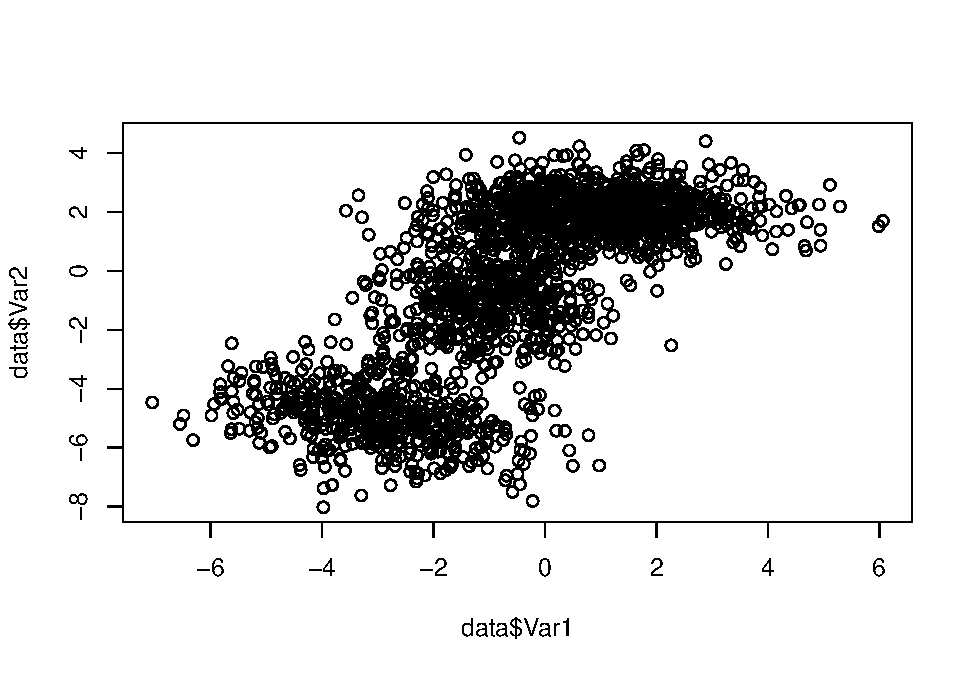
\includegraphics{539-hw3_files/figure-latex/unnamed-chunk-8-1.pdf} the
number of clusters is 3.

\hypertarget{b-2}{%
\subsection{b)}\label{b-2}}

\begin{Shaded}
\begin{Highlighting}[]
\FunctionTok{library}\NormalTok{(fMultivar)}
\end{Highlighting}
\end{Shaded}

\begin{verbatim}
## 载入需要的程辑包:timeDate
\end{verbatim}

\begin{verbatim}
## 载入需要的程辑包:timeSeries
\end{verbatim}

\begin{verbatim}
## 载入需要的程辑包:fBasics
\end{verbatim}

\begin{Shaded}
\begin{Highlighting}[]
\FunctionTok{msnFit}\NormalTok{(data)}
\end{Highlighting}
\end{Shaded}

\begin{verbatim}
## 
## Title:
##  Skew Normal Parameter Estimation 
## 
## Call:
##  msnFit(x = data)
## 
## Model:
##  Skew Normal Distribution
## 
## Estimated Parameter(s):
## $beta
##          Var1     Var2
## [1,] 1.455257 3.191867
## 
## $Omega
##           Var1     Var2
## Var1  8.146794 11.70847
## Var2 11.708474 22.46951
## 
## $alpha
##        Var1        Var2 
##  -0.8598872 -10.2055688 
## 
## 
## Description:
##  Mon Feb 28 19:08:23 2022 by user: 11193
\end{verbatim}

\begin{Shaded}
\begin{Highlighting}[]
\FunctionTok{library}\NormalTok{(ellipse)}
\end{Highlighting}
\end{Shaded}

\begin{verbatim}
## 
## 载入程辑包:'ellipse'
\end{verbatim}

\begin{verbatim}
## The following object is masked from 'package:graphics':
## 
##     pairs
\end{verbatim}

\begin{Shaded}
\begin{Highlighting}[]
\NormalTok{rho }\OtherTok{=} \FunctionTok{cor}\NormalTok{(data)}
\NormalTok{y\_on\_x }\OtherTok{\textless{}{-}} \FunctionTok{lm}\NormalTok{(data}\SpecialCharTok{$}\NormalTok{Var2 }\SpecialCharTok{\textasciitilde{}}\NormalTok{ data}\SpecialCharTok{$}\NormalTok{Var1)}
\NormalTok{x\_on\_y }\OtherTok{\textless{}{-}} \FunctionTok{lm}\NormalTok{(data}\SpecialCharTok{$}\NormalTok{Var1 }\SpecialCharTok{\textasciitilde{}}\NormalTok{ data}\SpecialCharTok{$}\NormalTok{Var2)}
\NormalTok{plot\_legend }\OtherTok{\textless{}{-}} \FunctionTok{c}\NormalTok{(}\StringTok{"99\% CI green"}\NormalTok{, }\StringTok{"95\% CI red"}\NormalTok{,}\StringTok{"90\% CI blue"}\NormalTok{,}
                 \StringTok{"Y on X black"}\NormalTok{, }\StringTok{"X on Y brown"}\NormalTok{)}
\FunctionTok{plot}\NormalTok{(data, }\AttributeTok{xlab =} \StringTok{"X"}\NormalTok{, }\AttributeTok{ylab =} \StringTok{"Y"}\NormalTok{,}\AttributeTok{col =} \StringTok{"grey"}\NormalTok{)}
\FunctionTok{lines}\NormalTok{(}\FunctionTok{ellipse}\NormalTok{(rho), }\AttributeTok{col=}\StringTok{"red"}\NormalTok{)}
\FunctionTok{lines}\NormalTok{(}\FunctionTok{ellipse}\NormalTok{(rho, }\AttributeTok{level =}\NormalTok{ .}\DecValTok{99}\NormalTok{), }\AttributeTok{col=}\StringTok{"green"}\NormalTok{)}
\FunctionTok{lines}\NormalTok{(}\FunctionTok{ellipse}\NormalTok{(rho, }\AttributeTok{level =}\NormalTok{ .}\DecValTok{90}\NormalTok{), }\AttributeTok{col=}\StringTok{"blue"}\NormalTok{)}
\FunctionTok{abline}\NormalTok{(y\_on\_x)}
\FunctionTok{abline}\NormalTok{(x\_on\_y, }\AttributeTok{col=}\StringTok{"brown"}\NormalTok{)}
\FunctionTok{legend}\NormalTok{(}\DecValTok{3}\NormalTok{,}\DecValTok{1}\NormalTok{,}\AttributeTok{legend=}\NormalTok{plot\_legend,}\AttributeTok{cex =}\NormalTok{ .}\DecValTok{5}\NormalTok{, }\AttributeTok{bty =} \StringTok{"n"}\NormalTok{)}
\end{Highlighting}
\end{Shaded}

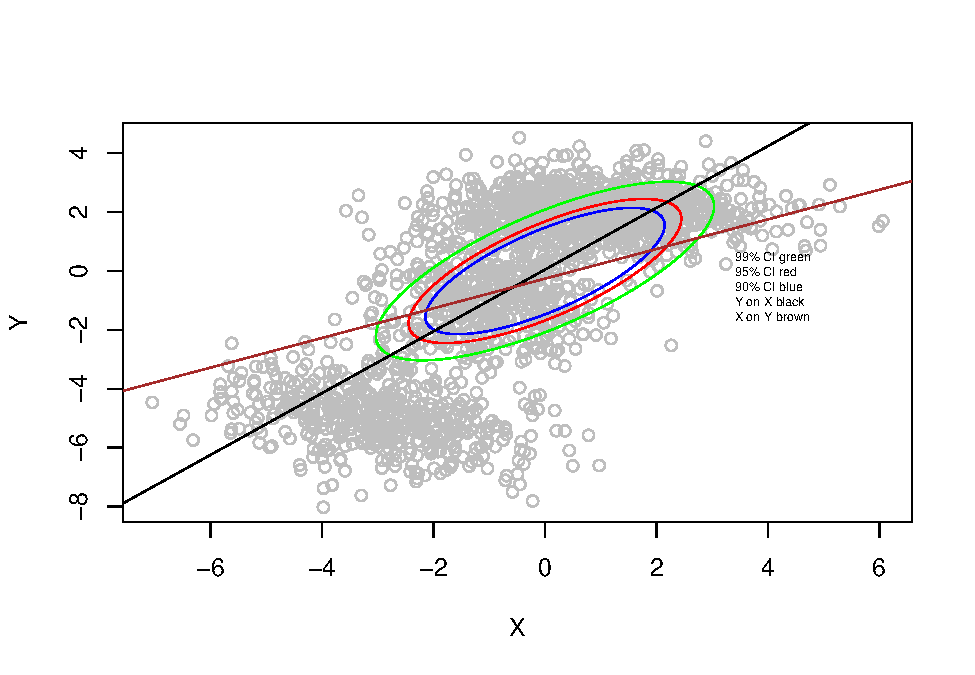
\includegraphics{539-hw3_files/figure-latex/unnamed-chunk-9-1.pdf} \#\#
c)

\begin{Shaded}
\begin{Highlighting}[]
\FunctionTok{library}\NormalTok{(MGMM)}
\NormalTok{d }\OtherTok{\textless{}{-}} \FunctionTok{as.matrix}\NormalTok{(data)}
\NormalTok{K2GMM }\OtherTok{\textless{}{-}} \FunctionTok{FitGMM}\NormalTok{(d,}\AttributeTok{k=}\DecValTok{2}\NormalTok{)}
\end{Highlighting}
\end{Shaded}

\begin{verbatim}
## Objective increment:  10.8 
## Objective increment:  0.793 
## Objective increment:  0.21 
## Objective increment:  0.184 
## Objective increment:  0.218 
## Objective increment:  0.27 
## Objective increment:  0.336 
## Objective increment:  0.418 
## Objective increment:  0.519 
## Objective increment:  0.644 
## Objective increment:  0.799 
## Objective increment:  0.99 
## Objective increment:  1.23 
## Objective increment:  1.52 
## Objective increment:  1.89 
## Objective increment:  2.35 
## Objective increment:  2.93 
## Objective increment:  3.67 
## Objective increment:  4.6 
## Objective increment:  5.77 
## Objective increment:  7.21 
## Objective increment:  8.89 
## Objective increment:  10.6 
## Objective increment:  12 
## Objective increment:  12.2 
## Objective increment:  10.8 
## Objective increment:  8.22 
## Objective increment:  5.53 
## Objective increment:  3.51 
## Objective increment:  2.22 
## Objective increment:  1.42 
## Objective increment:  0.928 
## Objective increment:  0.614 
## Objective increment:  0.411 
## Objective increment:  0.276 
## Objective increment:  0.187 
## Objective increment:  0.127 
## Objective increment:  0.0864 
## Objective increment:  0.059 
## Objective increment:  0.0403 
## Objective increment:  0.0276 
## Objective increment:  0.0189 
## Objective increment:  0.0129 
## Objective increment:  0.00888 
## Objective increment:  0.0061 
## Objective increment:  0.00419 
## Objective increment:  0.00288 
## Objective increment:  0.00198 
## Objective increment:  0.00136 
## Objective increment:  0.000935 
## Objective increment:  0.000643 
## Objective increment:  0.000442 
## Objective increment:  0.000304 
## Objective increment:  0.000209 
## Objective increment:  0.000144 
## Objective increment:  9.91e-05 
## Objective increment:  6.82e-05 
## Objective increment:  4.69e-05 
## Objective increment:  3.23e-05 
## Objective increment:  2.22e-05 
## Objective increment:  1.53e-05 
## Objective increment:  1.05e-05 
## Objective increment:  7.25e-06 
## Objective increment:  4.99e-06 
## Objective increment:  3.43e-06 
## Objective increment:  2.36e-06 
## Objective increment:  1.63e-06 
## Objective increment:  1.12e-06 
## Objective increment:  7.71e-07 
## 68 update(s) performed before reaching tolerance limit.
\end{verbatim}

\begin{Shaded}
\begin{Highlighting}[]
\FunctionTok{plot}\NormalTok{(data, }\AttributeTok{xlab =} \StringTok{"X"}\NormalTok{, }\AttributeTok{ylab =} \StringTok{"Y"}\NormalTok{,}\AttributeTok{col =} \StringTok{"grey"}\NormalTok{)}
\FunctionTok{points}\NormalTok{(K2GMM}\SpecialCharTok{@}\NormalTok{Means[[}\DecValTok{1}\NormalTok{]][}\DecValTok{1}\NormalTok{],K2GMM}\SpecialCharTok{@}\NormalTok{Means[[}\DecValTok{1}\NormalTok{]][}\DecValTok{2}\NormalTok{],}\AttributeTok{col =} \StringTok{"red"}\NormalTok{)}
\FunctionTok{points}\NormalTok{(K2GMM}\SpecialCharTok{@}\NormalTok{Means[[}\DecValTok{2}\NormalTok{]][}\DecValTok{1}\NormalTok{],K2GMM}\SpecialCharTok{@}\NormalTok{Means[[}\DecValTok{2}\NormalTok{]][}\DecValTok{2}\NormalTok{],}\AttributeTok{col =} \StringTok{"dark green"}\NormalTok{)}
\end{Highlighting}
\end{Shaded}

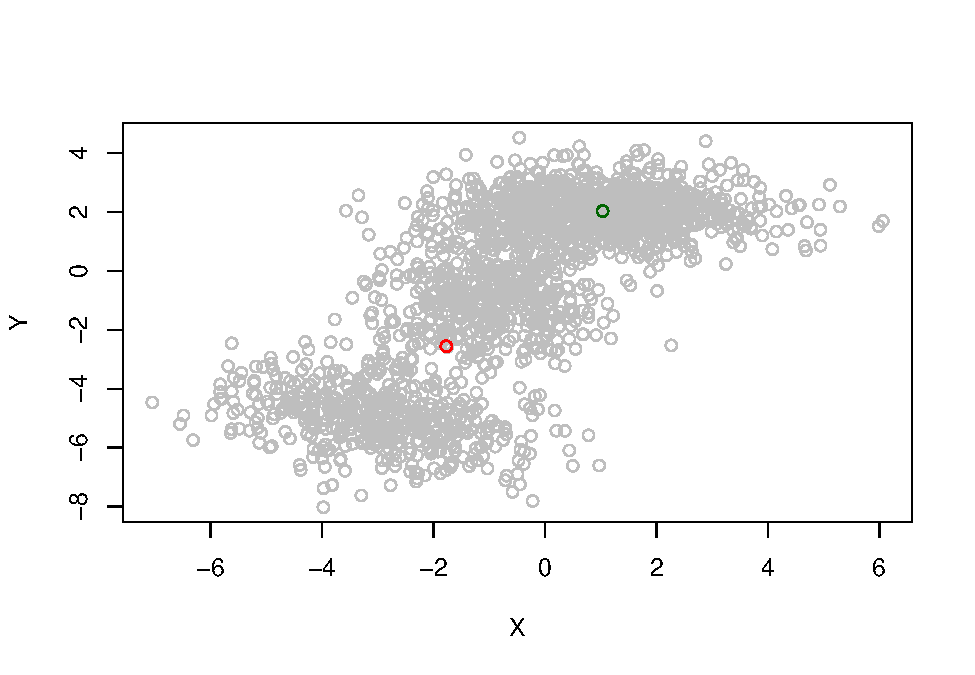
\includegraphics{539-hw3_files/figure-latex/unnamed-chunk-10-1.pdf} \#\#
d)

\begin{Shaded}
\begin{Highlighting}[]
\NormalTok{K3GMM }\OtherTok{\textless{}{-}} \FunctionTok{FitGMM}\NormalTok{(d,}\AttributeTok{k=}\DecValTok{3}\NormalTok{)}
\end{Highlighting}
\end{Shaded}

\begin{verbatim}
## Objective increment:  17.1 
## Objective increment:  3.64 
## Objective increment:  1.16 
## Objective increment:  0.414 
## Objective increment:  0.163 
## Objective increment:  0.0716 
## Objective increment:  0.0356 
## Objective increment:  0.02 
## Objective increment:  0.0126 
## Objective increment:  0.00851 
## Objective increment:  0.00604 
## Objective increment:  0.0044 
## Objective increment:  0.00325 
## Objective increment:  0.00241 
## Objective increment:  0.0018 
## Objective increment:  0.00134 
## Objective increment:  0.000998 
## Objective increment:  0.000743 
## Objective increment:  0.000553 
## Objective increment:  0.000412 
## Objective increment:  0.000306 
## Objective increment:  0.000228 
## Objective increment:  0.000169 
## Objective increment:  0.000126 
## Objective increment:  9.32e-05 
## Objective increment:  6.91e-05 
## Objective increment:  5.13e-05 
## Objective increment:  3.8e-05 
## Objective increment:  2.82e-05 
## Objective increment:  2.09e-05 
## Objective increment:  1.55e-05 
## Objective increment:  1.15e-05 
## Objective increment:  8.52e-06 
## Objective increment:  6.32e-06 
## Objective increment:  4.68e-06 
## Objective increment:  3.47e-06 
## Objective increment:  2.57e-06 
## Objective increment:  1.9e-06 
## Objective increment:  1.41e-06 
## Objective increment:  1.05e-06 
## Objective increment:  7.74e-07 
## 40 update(s) performed before reaching tolerance limit.
\end{verbatim}

\begin{Shaded}
\begin{Highlighting}[]
\FunctionTok{plot}\NormalTok{(data, }\AttributeTok{xlab =} \StringTok{"X"}\NormalTok{, }\AttributeTok{ylab =} \StringTok{"Y"}\NormalTok{,}\AttributeTok{col =} \StringTok{"grey"}\NormalTok{)}
\FunctionTok{points}\NormalTok{(K3GMM}\SpecialCharTok{@}\NormalTok{Means[[}\DecValTok{1}\NormalTok{]][}\DecValTok{1}\NormalTok{],K3GMM}\SpecialCharTok{@}\NormalTok{Means[[}\DecValTok{1}\NormalTok{]][}\DecValTok{2}\NormalTok{],}\AttributeTok{col =} \StringTok{"red"}\NormalTok{)}
\FunctionTok{points}\NormalTok{(K3GMM}\SpecialCharTok{@}\NormalTok{Means[[}\DecValTok{2}\NormalTok{]][}\DecValTok{1}\NormalTok{],K3GMM}\SpecialCharTok{@}\NormalTok{Means[[}\DecValTok{2}\NormalTok{]][}\DecValTok{2}\NormalTok{],}\AttributeTok{col =} \StringTok{"dark green"}\NormalTok{)}
\FunctionTok{points}\NormalTok{(K3GMM}\SpecialCharTok{@}\NormalTok{Means[[}\DecValTok{3}\NormalTok{]][}\DecValTok{1}\NormalTok{],K3GMM}\SpecialCharTok{@}\NormalTok{Means[[}\DecValTok{3}\NormalTok{]][}\DecValTok{2}\NormalTok{],}\AttributeTok{col =} \StringTok{"blue"}\NormalTok{)}
\end{Highlighting}
\end{Shaded}

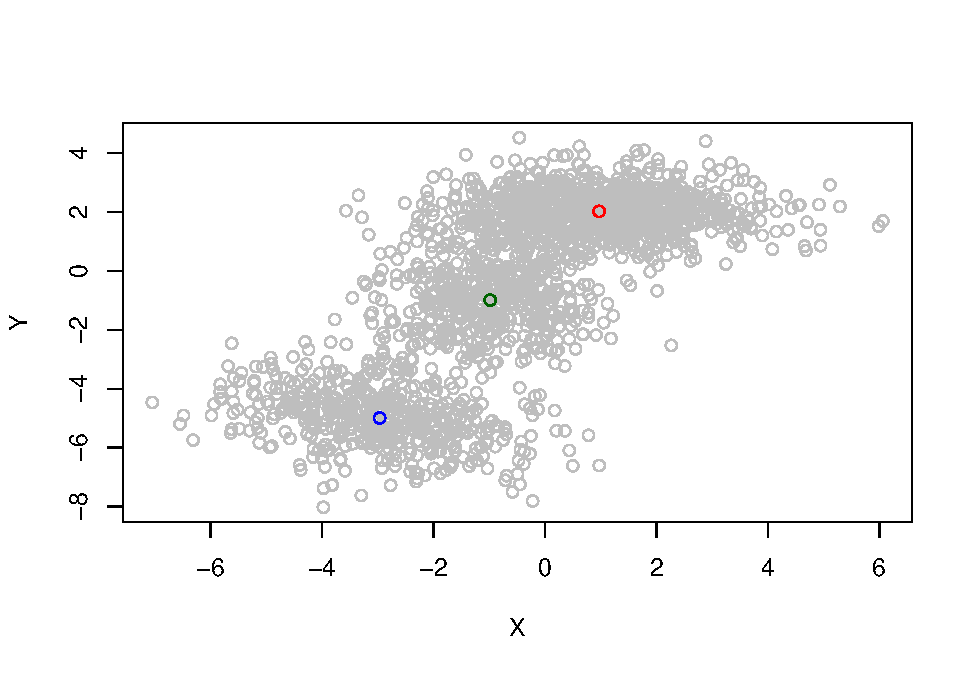
\includegraphics{539-hw3_files/figure-latex/unnamed-chunk-11-1.pdf} \#\#
e)

\begin{Shaded}
\begin{Highlighting}[]
\CommentTok{\# Sigma\_i = dx * d covariance matrix}
\NormalTok{si }\OtherTok{\textless{}{-}} \FunctionTok{diff}\NormalTok{(data}\SpecialCharTok{$}\NormalTok{Var1) }\SpecialCharTok{\%*\%} \FunctionTok{diff}\NormalTok{(rho)}
\NormalTok{si[}\DecValTok{1}\SpecialCharTok{:}\DecValTok{20}\NormalTok{,]}
\end{Highlighting}
\end{Shaded}

\begin{verbatim}
##             Var1       Var2
##  [1,]  0.2714496 -0.2714496
##  [2,]  0.7881399 -0.7881399
##  [3,]  0.7121274 -0.7121274
##  [4,] -0.8031689  0.8031689
##  [5,] -0.6439405  0.6439405
##  [6,] -0.3233667  0.3233667
##  [7,]  0.8456699 -0.8456699
##  [8,] -1.2999374  1.2999374
##  [9,]  1.1007313 -1.1007313
## [10,]  0.4108798 -0.4108798
## [11,]  0.1088834 -0.1088834
## [12,] -0.4082431  0.4082431
## [13,]  0.5513425 -0.5513425
## [14,] -0.1791793  0.1791793
## [15,]  0.5668767 -0.5668767
## [16,] -1.3834752  1.3834752
## [17,]  0.2978884 -0.2978884
## [18,] -0.1558065  0.1558065
## [19,]  1.0285411 -1.0285411
## [20,] -0.3159542  0.3159542
\end{verbatim}

\hypertarget{poisson-mixture-model}{%
\section{Poisson Mixture Model}\label{poisson-mixture-model}}

\hypertarget{section}{%
\subsection{1)}\label{section}}

\begin{Shaded}
\begin{Highlighting}[]
\FunctionTok{rm}\NormalTok{(}\AttributeTok{list =} \FunctionTok{ls}\NormalTok{())}
\end{Highlighting}
\end{Shaded}

\begin{Shaded}
\begin{Highlighting}[]
\FunctionTok{library}\NormalTok{(}\StringTok{"readxl"}\NormalTok{)}
\NormalTok{data }\OtherTok{\textless{}{-}} \FunctionTok{read\_excel}\NormalTok{(}\StringTok{"poisson\_data.xlsx"}\NormalTok{)}
\NormalTok{x }\OtherTok{\textless{}{-}}\NormalTok{ data}\SpecialCharTok{$}\NormalTok{X}
\FunctionTok{hist}\NormalTok{(x)}
\end{Highlighting}
\end{Shaded}

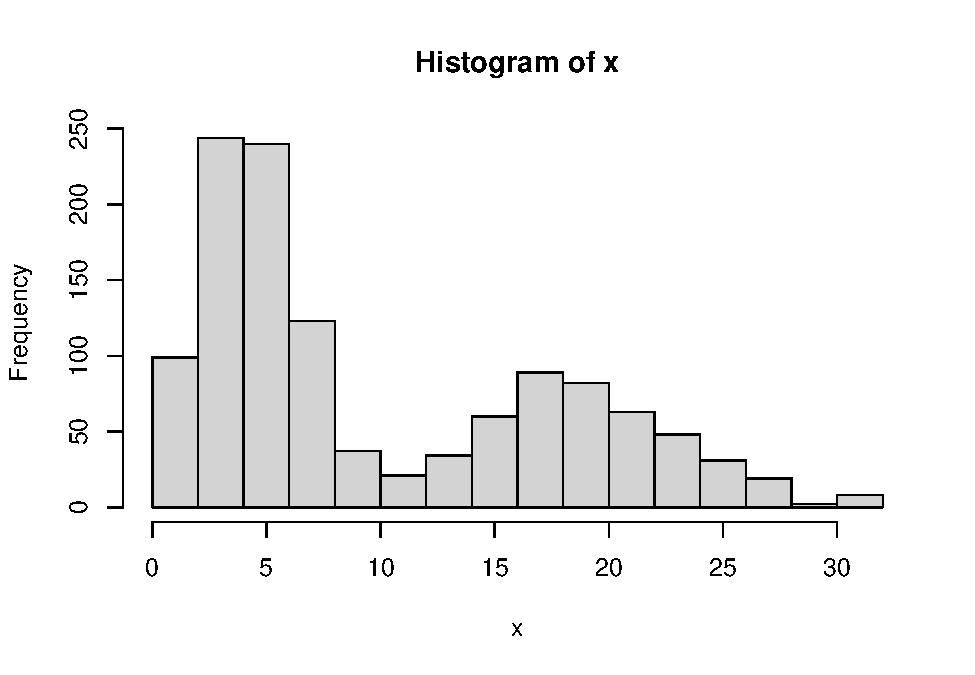
\includegraphics{539-hw3_files/figure-latex/unnamed-chunk-14-1.pdf} From
the plot it may fit two distribution from 1-10 and 10-30

\hypertarget{b-3}{%
\subsection{b)}\label{b-3}}

\begin{Shaded}
\begin{Highlighting}[]
\FunctionTok{library}\NormalTok{(MASS)}
\NormalTok{lambda }\OtherTok{\textless{}{-}} \FunctionTok{fitdistr}\NormalTok{(x,}\AttributeTok{densfun=}\StringTok{"Poisson"}\NormalTok{)}
\NormalTok{lambda}
\end{Highlighting}
\end{Shaded}

\begin{verbatim}
##      lambda   
##   10.37833333 
##  ( 0.09299791)
\end{verbatim}

\begin{Shaded}
\begin{Highlighting}[]
\NormalTok{a }\OtherTok{\textless{}{-}} \DecValTok{0}\SpecialCharTok{:}\DecValTok{30}
\NormalTok{b }\OtherTok{\textless{}{-}} \FunctionTok{dpois}\NormalTok{(a,lambda}\SpecialCharTok{$}\NormalTok{estimate)}
\FunctionTok{hist}\NormalTok{(x,}\AttributeTok{xlim=}\FunctionTok{c}\NormalTok{(}\DecValTok{0}\NormalTok{,}\DecValTok{30}\NormalTok{),}\AttributeTok{ylim=} \FunctionTok{c}\NormalTok{(}\DecValTok{0}\NormalTok{,}\DecValTok{250}\NormalTok{))}
\FunctionTok{par}\NormalTok{(}\AttributeTok{new=}\ConstantTok{TRUE}\NormalTok{)}
\FunctionTok{plot}\NormalTok{(a,b,}\AttributeTok{yaxt=}\StringTok{"n"}\NormalTok{,}\AttributeTok{xaxt=}\StringTok{"n"}\NormalTok{,}\AttributeTok{xlab=}\StringTok{""}\NormalTok{,}\AttributeTok{ylab=}\StringTok{""}\NormalTok{)}
\end{Highlighting}
\end{Shaded}

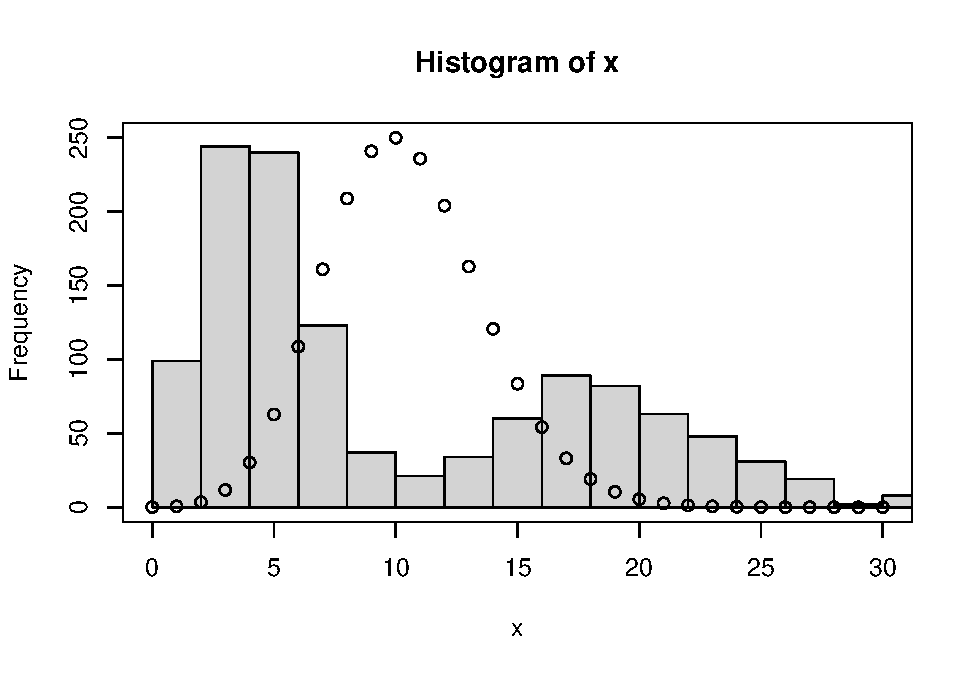
\includegraphics{539-hw3_files/figure-latex/unnamed-chunk-15-1.pdf} a
simple poisson distribution is not a good fit.

\hypertarget{c-2}{%
\subsection{c)}\label{c-2}}

\begin{Shaded}
\begin{Highlighting}[]
\FunctionTok{library}\NormalTok{(mixtools)}
\end{Highlighting}
\end{Shaded}

\begin{verbatim}
## mixtools package, version 1.2.0, Released 2020-02-05
## This package is based upon work supported by the National Science Foundation under Grant No. SES-0518772.
\end{verbatim}

\begin{verbatim}
## 
## 载入程辑包:'mixtools'
\end{verbatim}

\begin{verbatim}
## The following object is masked from 'package:ellipse':
## 
##     ellipse
\end{verbatim}

\begin{Shaded}
\begin{Highlighting}[]
\NormalTok{mixture }\OtherTok{\textless{}{-}} \FunctionTok{normalmixEM}\NormalTok{(x,}\AttributeTok{lambda =} \FloatTok{0.092997}\NormalTok{,}\AttributeTok{k=}\DecValTok{2}\NormalTok{)}
\end{Highlighting}
\end{Shaded}

\begin{verbatim}
## number of iterations= 19
\end{verbatim}

\begin{Shaded}
\begin{Highlighting}[]
\FunctionTok{summary}\NormalTok{(mixture)}
\end{Highlighting}
\end{Shaded}

\begin{verbatim}
## summary of normalmixEM object:
##          comp 1    comp 2
## lambda 0.604878  0.395122
## mu     4.722446 19.036704
## sigma  2.052661  4.708311
## loglik at estimate:  -3707.207
\end{verbatim}

\hypertarget{d-1}{%
\subsection{d)}\label{d-1}}

\begin{Shaded}
\begin{Highlighting}[]
\FunctionTok{plot}\NormalTok{(mixture, }\AttributeTok{density=}\ConstantTok{TRUE}\NormalTok{)}
\end{Highlighting}
\end{Shaded}

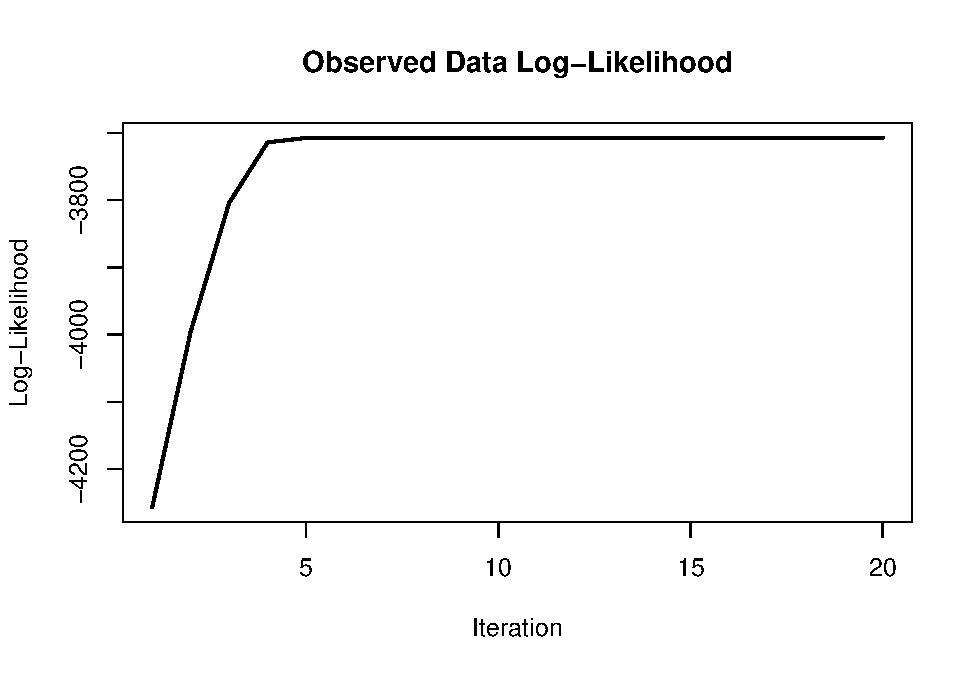
\includegraphics{539-hw3_files/figure-latex/unnamed-chunk-17-1.pdf}
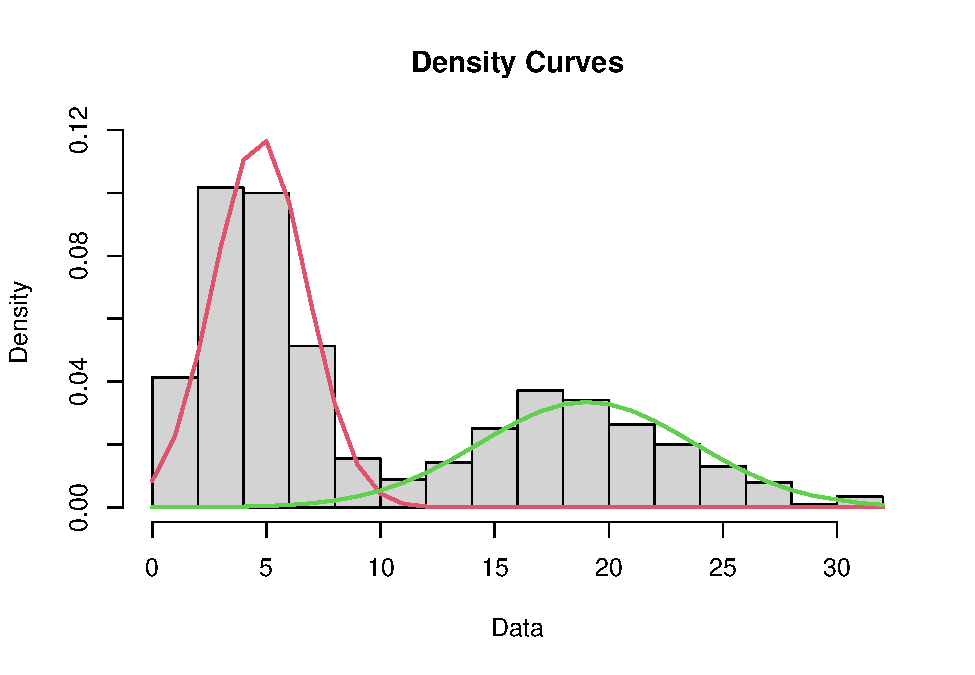
\includegraphics{539-hw3_files/figure-latex/unnamed-chunk-17-2.pdf}

\hypertarget{e}{%
\subsection{e)}\label{e}}

the single poisson distribution can not fit the data very well, the
mixture model give two poisson distribution and separate the data into
two modle, which fit the data better.

\end{document}
